\documentclass[aps,pra,twocolumn,reprint,amsmath,amssymb]{revtex4-2}

\usepackage{graphicx}
\usepackage{booktabs}
\usepackage{siunitx}
\usepackage[colorlinks=true,linkcolor=blue,citecolor=blue,urlcolor=blue]{hyperref}

\usepackage{xcolor}
\graphicspath{{../figures/}}

\begin{document}

\title{Dispersive Readout Pulse Optimization in Circuit QED:
From Linear Theory to Hardware-Realistic QND Limits and Leakage Mapping}
\author{cQED Autonomous Research Platform}
\affiliation{Shyam Shankar Quantum Circuits Group}
\date{\today}

% ══════════════════════════════════════════════════════════
% 1. ABSTRACT
% ══════════════════════════════════════════════════════════
\begin{abstract}
We present a unified study of dispersive readout pulse optimization in circuit quantum electrodynamics, covering the full model-refinement chain from linear dispersive theory through multilevel transmon dynamics, hardware-realistic waveform transport, nonlinear QND modeling, and high-power leakage/ionization mapping. Four progressive investigations are consolidated into a single analysis for a representative transmon--readout-resonator system with $\omega_q/2\pi=\SI{6.150}{GHz}$, $\omega_r/2\pi=\SI{8.597}{GHz}$, $\chi/2\pi=\SI{-2.84}{MHz}$, $\kappa/2\pi=\SI{2.4}{MHz}$, and $\alpha/2\pi=\SI{-255}{MHz}$.

The main results span four model levels: (1)~In the linear dispersive model, the midpoint-driven square pulse is optimal under peak-amplitude constraints, and GRAPE does not improve upon it. (2)~In the multilevel \texttt{cqed\_sim} replay, structured procedural pulses recover most of the information-theoretic bound while dramatically reducing residual photons: the best free procedural family reaches $F_\eta=0.956$ at \SI{240}{ns} compared with $0.871$ for a square pulse. (3)~Under hardware-realistic waveform transport and phenomenological strong-drive QND penalties, the ring-up/hold/ring-down family emerges as the best practical default, with $F_\eta=0.9599$ at \SI{240}{ns} and superior QND preservation. (4)~At high readout power, visible leakage appears above $\varepsilon/(2\pi)\approx\SI{5.5}{MHz}$ for \SI{240}{ns} pulses, with QND breakdown dominating over high-manifold ionization. The combined analysis provides actionable recommendations for experiment-facing readout pulse design.
\end{abstract}

\maketitle

% ══════════════════════════════════════════════════════════
% 2. INTRODUCTION
% ══════════════════════════════════════════════════════════
\section{Introduction}

Dispersive readout is the canonical method for measuring superconducting qubits in the circuit QED architecture~\cite{blais2021circuit,krantz2019quantum}. A microwave tone drives a readout resonator coupled dispersively to the qubit; the qubit-state-dependent resonator response encodes the qubit state in the phase and amplitude of the output field. While the physics of dispersive readout is well understood~\cite{gambetta2007protocols,boissonneault2009dispersive}, the optimal control of the readout pulse shape has received less systematic attention than gate pulse design.

Three practical requirements compete: (i)~\emph{fast} readout (large signal-to-noise ratio per unit time), (ii)~\emph{clean} reset (minimal residual resonator photons after readout), and (iii)~\emph{QND} character (minimal qubit disturbance during readout). Optimizing these simultaneously calls for a carefully chosen objective function, waveform class, and physical model. Active resonator reset~\cite{mcclure2016rapid} and fast readout by waveform shaping~\cite{walter2017rapid,jeffrey2014fast} have been demonstrated experimentally, but a systematic comparison across progressive model complexity has been lacking.

\paragraph{Experiment-facing question.}
The practical question is not simply ``which pulse maximizes assignment fidelity in simulation?'' It is: \emph{which pulse family should an experimentalist calibrate first, which tradeoff curve actually matters on hardware, and when does the weak-drive dispersive picture stop being predictive?} We therefore organize the study around decisions a lab would make in practice: which family best balances fidelity, cavity emptying, and QND preservation; how close one can safely push toward the high-power frontier; and when a more advanced driven multilevel or Floquet-style analysis becomes justified.

This unified study fills that gap through four progressive investigations. Section~\ref{sec:linear} establishes the linear dispersive baseline: GRAPE versus analytical pulse families, midpoint drive optimality, and objective function selection. Section~\ref{sec:procedural} introduces structured procedural pulse families (ring-hold, free segments, analytic nulling tails) evaluated in the multilevel \texttt{cqed\_sim} model. Section~\ref{sec:hardware} adds hardware-realistic waveform transport and a phenomenological strong-drive QND penalty, revealing that the ring-hold family becomes the best practical default. Section~\ref{sec:leakage} extends the model to map leakage and ionization regimes at high readout power with an extended transmon (5~levels, 18~Fock states). Section~\ref{sec:validation} presents the validation checks, and the study concludes with a practical recommendation table and a detailed limitations analysis.

% ══════════════════════════════════════════════════════════
% 3. SYSTEM & METHODS
% ══════════════════════════════════════════════════════════
\section{System and Methods}

\subsection{Hamiltonian}

All four model levels share the same underlying device parameters but differ in the operator structure and dissipation channels included.

\paragraph{Level 0: Linear dispersive model.}
In the frame rotating at the drive frequency $\omega_d$, the qubit-state-conditioned resonator coherent amplitude $\alpha_j(t)$ ($j\in\{g,e\}$) obeys
\begin{equation}
\dot{\alpha}_j = -\left(\frac{\kappa}{2} + i\Delta_j\right)\alpha_j - i\varepsilon(t),
\label{eq:linear_ode}
\end{equation}
where $\Delta_g = \omega_r - \omega_d$, $\Delta_e = \omega_r + \chi - \omega_d$, and $\varepsilon(t)$ is the complex drive envelope. The output field is $s_j(t) = \sqrt{\kappa}\,\alpha_j(t)$.

\paragraph{Level 1: Multilevel dispersive model.}
The replay uses the two-mode multilevel Hamiltonian supported by \texttt{cqed\_sim}:
\begin{equation}
\frac{H_0}{\hbar} = \delta_c a^\dagger a + \delta_q b^\dagger b + \frac{\alpha}{2}b^{\dagger 2}b^2 + \frac{K}{2}a^{\dagger 2}a^2 + \chi\,a^\dagger a\,b^\dagger b,
\label{eq:multilevel_H}
\end{equation}
with cavity operator $a$, transmon operator $b$, and dissipation through \texttt{NoiseSpec}$(T_1, T_\phi, \kappa)$.

\paragraph{Level 2: Hardware-realistic model.}
The Level~1 Hamiltonian is augmented with hardware waveform transport (\texttt{SequenceCompiler(hardware=...)}) and an effective mixing layer that maps occupancy- and slew-dependent readout backaction onto explicit multilevel transition drives:
\begin{equation}
\frac{H_\mathrm{drive}}{\hbar} = \varepsilon_c(t)a^\dagger + \varepsilon_c^*(t)a + \Omega_{ge}(t)\sigma_{ge}^\dagger + \Omega_{ge}^*(t)\sigma_{ge} + \Omega_{ef}(t)\sigma_{ef}^\dagger + \Omega_{ef}^*(t)\sigma_{ef}.
\end{equation}

\paragraph{Level 3: Extended transmon for leakage mapping.}
The Level~2 model is extended to 5~transmon levels and 18~cavity Fock states, with the occupancy-activated disturbance continued to higher ladder transitions:
\begin{equation}
\frac{H_\mathrm{dist}(t)}{\hbar} = \varepsilon_{ge}(t)\sigma_{ge}^+ + \varepsilon_{ef}(t)\sigma_{ef}^+ + \sum_{m\ge 2}\lambda_m\varepsilon_{ef}(t)\sigma_{m,m+1}^+ + \mathrm{h.c.}
\end{equation}

\subsection{Simulation Parameters}

\begin{table*}[tp]
\centering
\caption{Nominal system parameters shared across all model levels.}
\begin{tabular}{@{} l S[table-format=+3.3] l @{}}
\toprule
Parameter & {Value} & Unit \\
\midrule
Qubit frequency $\omega_q/2\pi$ & 6.150 & GHz \\
Readout frequency $\omega_r/2\pi$ & 8.597 & GHz \\
Anharmonicity $\alpha/2\pi$ & -255 & MHz \\
Dispersive shift $\chi/2\pi$ & -2.84 & MHz \\
Resonator linewidth $\kappa/2\pi$ & 2.4 & MHz \\
Cavity self-Kerr $K/2\pi$ & -28 & kHz \\
Qubit $T_{1,ge}$ & 30 & $\mu$s \\
Qubit $T_{1,ef}$ & 12 & $\mu$s \\
Qubit $T_\phi$ & 30 & $\mu$s \\
Thermal occupation $n_\mathrm{th}$ & 0.015 & --- \\
Detector efficiency $\eta$ & 0.35 & --- \\
Time step $\Delta t$ & 4 & ns \\
Max drive amplitude $|\varepsilon_\mathrm{max}|/2\pi$ & 4.0 & MHz \\
Critical photon number $n_\mathrm{crit}$ & 20.3 & photons \\
\bottomrule
\end{tabular}
\label{tab:params}
\end{table*}

\begin{table*}[tp]
\centering
\caption{Model-level-specific parameters.}
\begin{tabular}{@{} l l l l l @{}}
\toprule
Parameter & Level 0 & Level 1 & Level 2 & Level 3 \\
\midrule
Transmon truncation & --- & 3 & 3 & 5 \\
Cavity truncation & --- & 14 & 14 & 18 \\
Hardware transport & No & No & Yes & Yes \\
QND mixing layer & No & No & Yes & Yes \\
LP bandwidth (MHz) & --- & --- & 75 & 75 \\
IQ gain ratio & --- & --- & 0.94 & --- \\
Mixing onset $n/n_\mathrm{crit}$ & --- & --- & 0.10 & 0.10 \\
$ge$ mixing scale & --- & --- & 0.09 & 0.09 \\
$ef$ mixing scale & --- & --- & 0.05 & 0.05 \\
\bottomrule
\end{tabular}
\label{tab:model_levels}
\end{table*}

\subsection{Pulse Families}

Seven pulse families are compared across the model hierarchy:
\begin{enumerate}
\item \textbf{Square}: constant-amplitude drive at the midpoint frequency.
\item \textbf{Gaussian}: truncated Gaussian envelope, area-normalized.
\item \textbf{Hann / cosine-rise}: smooth turn-on/off envelopes.
\item \textbf{Ring-up/hold/ring-down (ring-hold)}: three-segment structure with optimizable durations and amplitudes.
\item \textbf{Free procedural segments}: three independently optimized complex segments.
\item \textbf{Analytic nulling tail}: readout body followed by algebraically computed two-segment tail that drives $\alpha_g(T)=\alpha_e(T)=0$.
\item \textbf{Fourier basis}: smooth waveform expressed as a truncated Fourier series.
\end{enumerate}
Additionally, a high-dimensional piecewise-constant reference (8--10~segments) is used as an information-theoretic benchmark, and GRAPE~\cite{khaneja2005optimal} with 60~piecewise-constant segments provides an upper bound in the linear model.

\subsection{Computational Approach}

The primary practical objective is a balanced score:
\begin{equation}
J_\mathrm{bal} = F_\eta - 0.08\,n_\mathrm{res} - 0.70(1 - Q_\mathrm{QND}) - 1.20\,L,
\label{eq:balanced_score}
\end{equation}
where $F_\eta$ is the detector-limited matched-filter assignment fidelity, $n_\mathrm{res}$ is the mean residual photon number, $Q_\mathrm{QND}$ is the average state-preservation probability under repeated readout, and $L$ is leakage. The time-integrated SNR$^2$,
\begin{equation}
\mathrm{SNR}^2 = \kappa\int_0^T|\alpha_e(t) - \alpha_g(t)|^2\,dt,
\label{eq:snr2}
\end{equation}
serves as the information-only objective in the linear model.

% ══════════════════════════════════════════════════════════
% 4. RESULTS
% ══════════════════════════════════════════════════════════
\section{Results}

\subsection{Level 0: Linear Dispersive Baseline}
\label{sec:linear}

\paragraph{Midpoint drive optimality.}
The steady-state pointer separation is maximized at the midpoint drive $\omega_d = \omega_r + \chi/2$:
\begin{equation}
|\Delta\alpha^\mathrm{ss}_\mathrm{max}| = \frac{4|\varepsilon||\chi|}{\kappa^2 + \chi^2},
\end{equation}
which peaks at $|\chi/\kappa|=1$ with value $2|\varepsilon|/\kappa$. This is confirmed numerically to better than $10^{-6}$ relative error and agrees with \texttt{cqed\_sim.ReadoutResonator} to machine precision.

\paragraph{Objective function selection.}
The time-integrated SNR$^2$ (Eq.~\ref{eq:snr2}) is the most physically grounded single objective. Endpoint pointer separation ($J_A$) saturates prematurely and is a poor proxy for assignment fidelity at intermediate $\kappa T$.

\paragraph{GRAPE vs.\ analytical families.}
Under a shared peak-amplitude bound $|\varepsilon_k| \le |\varepsilon_\mathrm{max}|$, GRAPE (60~segments, L-BFGS-B, 10 random restarts) converges to the same square-like solution within numerical precision across $|\chi|/\kappa \in \{0.25, 0.5, 1.0, 2.0, 4.0\}$. The \textbf{midpoint-driven square pulse is optimal} in this linear, peak-limited setting. Among smooth families, the cosine-rise is competitive but never exceeds the square, while Gaussian, Hann, and spline envelopes underperform because they under-utilize the peak drive budget. The optimal duration including $T_1$-induced infidelity is $\kappa T \approx 5.79$ ($T\approx\SI{184}{ns}$ for $\kappa/2\pi=\SI{5}{MHz}$), yielding $F_\mathrm{net}^\mathrm{max}=0.9967$.

\paragraph{Active depletion (negative result).}
The implemented single-segment active-depletion heuristic does not outperform passive ring-down in the linear model and is not a useful control primitive in this setting.

\subsection{Level 1: Multilevel Procedural Optimization}
\label{sec:procedural}

\paragraph{Bound hierarchy.}
The high-dimensional piecewise linear reference reaches near-perfect detector-limited fidelity ($0.985$) by \SI{240}{ns} but leaves $n_\mathrm{res}=5.57$ photons, making it impractical. This establishes that information extraction is not the limiting factor beyond a few hundred nanoseconds; the design problem is retaining information while enforcing cavity emptying and QND character.

\paragraph{Structured families vs.\ square baseline.}
At the representative \SI{240}{ns} duration, structured procedural families dramatically outperform the square baseline:

\begin{table*}[tp]
\centering
\caption{Representative \SI{240}{ns} comparison in the multilevel model.}
\begin{tabular}{@{} l c c c c @{}}
\toprule
Family & $F_\eta$ & $n_\mathrm{res}$ & $Q_\mathrm{rep}$ \\
\midrule
Square & 0.871 & 1.485 & 0.853 \\
Ring-hold & 0.947 & 0.554 & 0.928 \\
Procedural segments & 0.956 & 0.620 & 0.950 \\
Nulled tail & 0.944 & 0.265 & 0.936 \\
Fourier basis & 0.953 & 0.721 & 0.938 \\
Piecewise reference (linear) & 0.985 & 5.572 & 0.979 \\
\bottomrule
\end{tabular}
\label{tab:level1_comparison}
\end{table*}

\paragraph{Analytic nulling.}
In the linear model, two free complex tail segments are sufficient to impose $\alpha_g(T)=\alpha_e(T)=0$ exactly, provided their durations are fixed and amplitudes satisfy the hardware cap. In realistic replay the nulling is approximate but effective: at \SI{336}{ns} the nulled family reaches $F_\eta=0.990$ with only $4.5\times 10^{-2}$ residual photons. At \SI{496}{ns}, $F_\eta=0.9995$ with $3.6\times 10^{-3}$ residual photons. Active emptying thus costs modest additional time.

\subsection{Level 2: Hardware-Realistic Readout with QND Penalties}
\label{sec:hardware}

\paragraph{Family reordering under the rich model.}
Once hardware transport and nonlinear QND penalties are included, the ring-hold family leads the frontier at all tested durations (\SIlist{96;240;496}{ns}). This is the central result: low-dimensional procedural structure survives, but the family with the most freedom is no longer the best default.

\begin{table*}[tp]
\centering
\caption{Representative \SI{240}{ns} hardware-realistic (rich model) comparison.}
\small
\begin{tabular}{@{} l c c c c c @{}}
\toprule
Family & $F_\eta$ & $n_\mathrm{res}$ & $Q_\mathrm{QND}$ & $p_\mathrm{ind}$ & $n_\mathrm{peak}$ \\
\midrule
Square & 0.9201 & 2.366 & 0.9931 & $1.94\times 10^{-4}$ & 3.156 \\
\textbf{Ring-hold} & \textbf{0.9599} & \textbf{0.801} & \textbf{0.9921} & $1.23\times 10^{-3}$ & 4.417 \\
Procedural segments & 0.9547 & 0.713 & 0.9886 & $4.66\times 10^{-3}$ & 3.999 \\
Nulling tail & 0.9216 & 0.887 & 0.9931 & $2.20\times 10^{-4}$ & 3.356 \\
Fourier basis & 0.9347 & 0.673 & 0.9931 & $2.35\times 10^{-4}$ & 2.925 \\
Piecewise ref.\ (bal.) & 0.9092 & 0.416 & 0.9933 & $4.09\times 10^{-5}$ & 3.098 \\
\bottomrule
\end{tabular}
\normalsize
\label{tab:level2_comparison}
\end{table*}

\paragraph{Transport vs.\ QND decomposition.}
For the procedural-segments design at \SI{240}{ns}: hardware transport alone lowers fidelity from $0.9628$ to $0.9552$ with no extra disturbance. The nonlinear layer alone leaves fidelity at $0.9625$ but reduces QND preservation from $0.9933$ to $0.9898$ through $p_\mathrm{ind}=3.51\times 10^{-3}$. The full rich model combines both effects ($F_\eta=0.9547$, $Q_\mathrm{QND}=0.9886$). This decomposition explains the ranking change: hardware transport punishes sharp envelopes, while the nonlinear channel punishes high-occupancy excursions. Ring-hold is smooth enough to survive the first and conservative enough to avoid the second.

\paragraph{QND stress test.}
At $1.3\times$ nominal amplitude, procedural segments fall to $Q_\mathrm{QND}=0.9618$ with $p_\mathrm{ind}=3.15\times 10^{-2}$, while Fourier basis remains at $Q_\mathrm{QND}=0.9890$. The most flexible family is the most stress-sensitive.

Figure~\ref{fig:family_tradeoffs} summarizes the most experimentally relevant comparison at \SI{240}{ns}. Level~1 shows what is possible once multilevel physics and cavity emptying are included, while Level~2 shows what survives once waveform transport and strong-drive disturbance are added. The visual message is the same as the tabulated one: the frontier moves toward smoother, more structured families as the model becomes closer to the lab.

\begin{figure*}[tp]
\centering
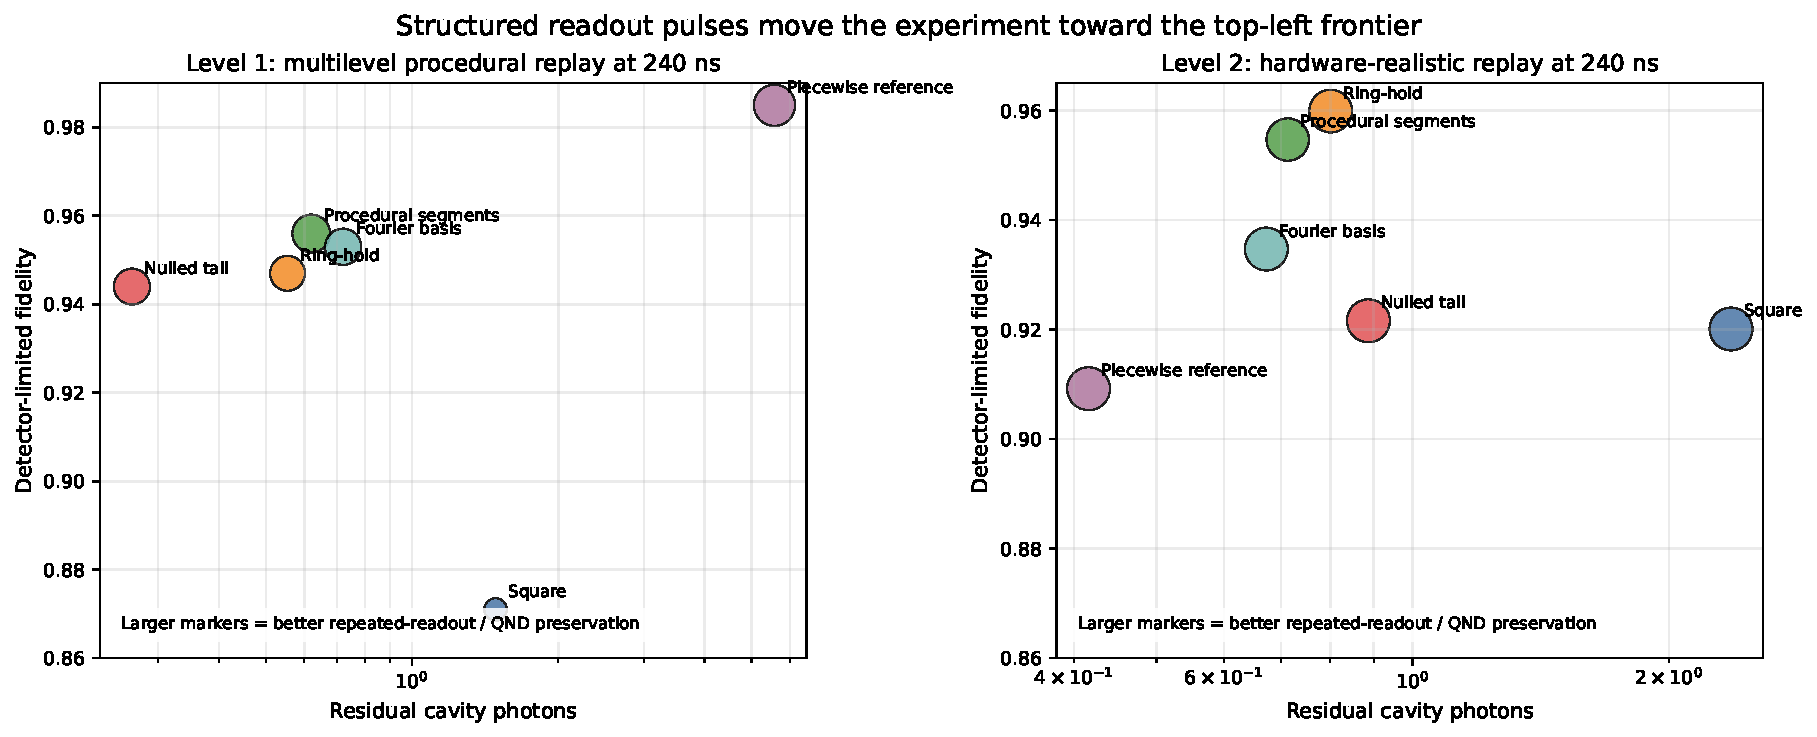
\includegraphics[width=\textwidth]{readout_family_tradeoffs.pdf}
\caption{Experiment-facing frontier at the representative \SI{240}{ns} operating point. Left: multilevel replay. Right: hardware-realistic replay with QND penalties. In both panels, moving toward the upper-left corresponds to better assignment fidelity with fewer residual photons, and larger markers indicate better repeated-readout preservation. The ring-hold family is the best practical frontier point once hardware transport and QND penalties are included.}
\label{fig:family_tradeoffs}
\end{figure*}

\subsection{Level 3: Leakage and Ionization Mapping}
\label{sec:leakage}

\paragraph{Regime maps.}
Using the extended transmon model (5~levels, 18~Fock states), the amplitude-duration regime map reveals a clear hierarchy: at the $P_\mathrm{leak}>10^{-4}$ benchmark, the threshold amplitude is approximately \SI{7.5}{MHz} at \SI{120}{ns}, \SI{5.5}{MHz} at \SI{240}{ns}, and \SI{4.5}{MHz} at \SI{480}{ns}. The threshold moves to lower power as pulse duration increases.

\paragraph{QND breakdown precedes ionization.}
The most severe tested point (\SI{480}{ns}, \SI{7.5}{MHz}) reaches $P_\mathrm{leak}=2.18\times 10^{-3}$ but only $P_\mathrm{ion}=1.25\times 10^{-6}$, with repeated-readout defect $0.495$. QND breakdown and nearby-level leakage are the dominant failure modes; broad high-manifold ionization remains negligible throughout the stable production window.

\paragraph{Detuning dependence.}
At the representative near-threshold point (\SI{240}{ns}), moving the drive from $-\SI{1.0}{MHz}$ to $+\SI{1.0}{MHz}$ relative to cavity resonance reduces $P_\mathrm{leak}$ from $1.91\times 10^{-4}$ to $4.65\times 10^{-5}$. The cavity-resonant point remains least damaging for repeated-readout consistency.

\paragraph{Mitigation.}
At fixed detector-limited fidelity target, smoother envelopes (Gaussian) leave only $0.053$ residual photons compared with $0.216$ for the square pulse. Fidelity saturates early in the detector-limited proxy; smoother envelopes mainly reduce residual cavity population rather than improving assignment.

Figure~\ref{fig:readout_window} translates the high-power study into experimental operating guidance. The leakage threshold shifts downward as pulse duration increases, over-driving penalizes flexible procedural pulses more strongly than smooth Fourier-like ones, and smoother envelopes mainly buy faster cavity emptying once the information-extraction proxy is already saturated.

\begin{figure*}[tp]
\centering
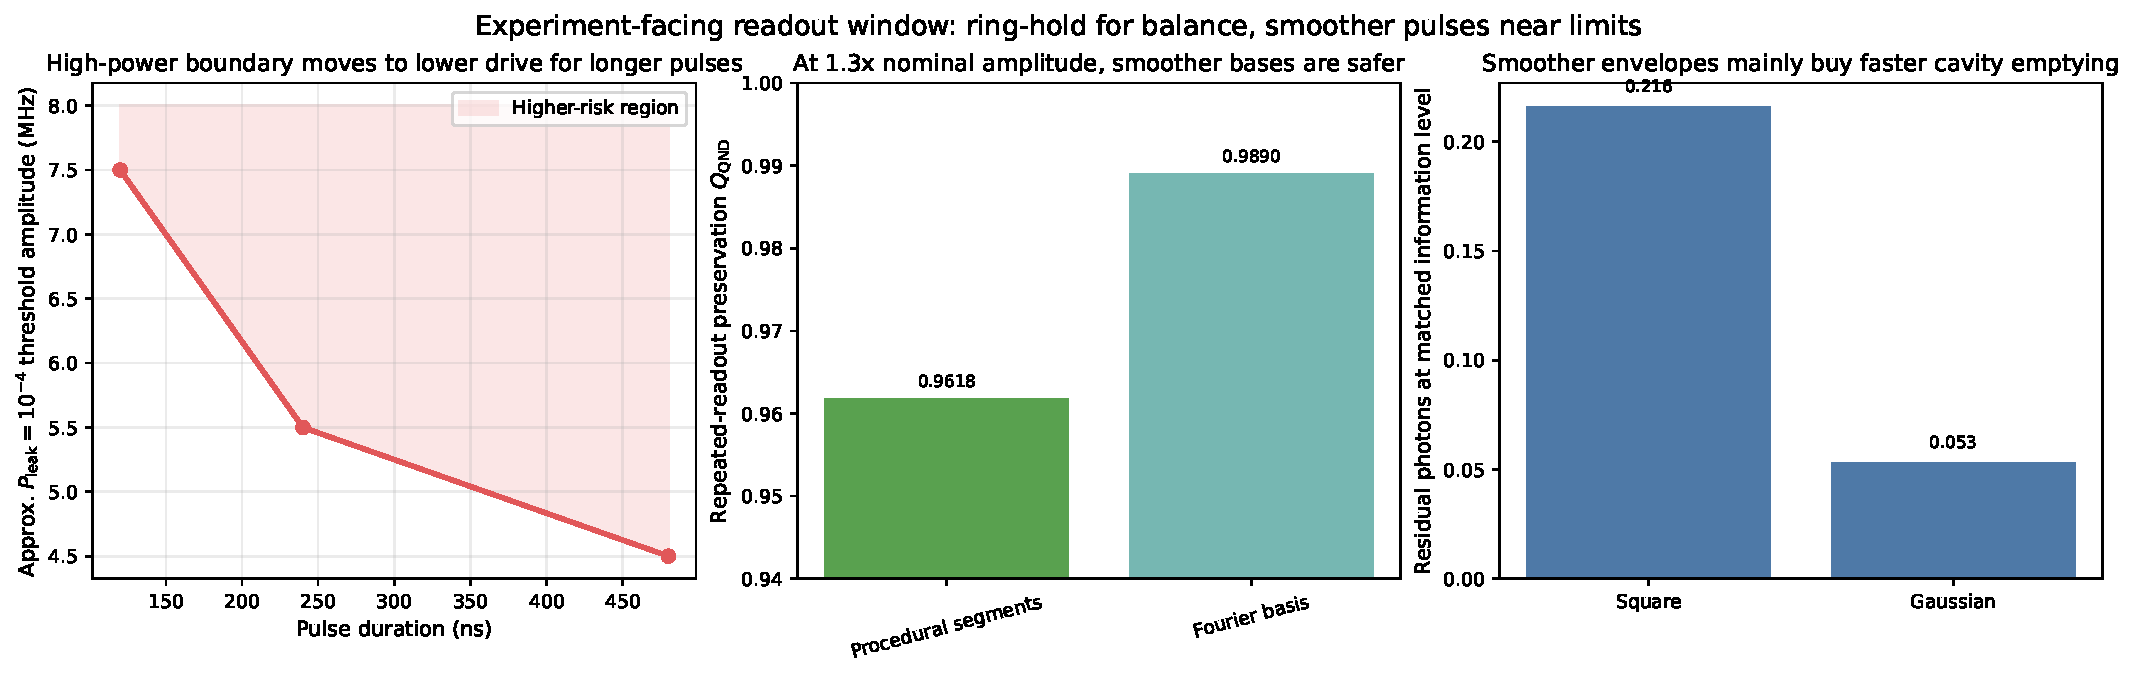
\includegraphics[width=\textwidth]{readout_operating_window.pdf}
\caption{High-power operating guidance for readout design. Left: approximate amplitude at which $P_\mathrm{leak}\approx 10^{-4}$ versus pulse duration. Middle: repeated-readout preservation under a $1.3\times$ over-drive stress test. Right: residual photons at matched detector-limited fidelity. The experimentally relevant message is that the safe operating window shrinks with pulse duration, and smoother families help most when cavity emptying or QND margin is the bottleneck.}
\label{fig:readout_window}
\end{figure*}

% ══════════════════════════════════════════════════════════
% 5. VALIDATION
% ══════════════════════════════════════════════════════════
\section{Validation}
\label{sec:validation}

\subsection{Sanity Checks}
All model levels satisfy basic sanity requirements. The analytic midpoint-drive formula agrees with \texttt{cqed\_sim.ReadoutResonator} to machine precision. The nulling-tail construction drives both conditioned linear cavity amplitudes to zero exactly. Low-power limits show negligible leakage and expected repeated-readout consistency ($0.989$ at \SI{1.5}{MHz}, \SI{120}{ns}). Peak occupancy and leakage increase monotonically across amplitude sweeps.

\subsection{Convergence Analysis}
At the representative near-threshold point (\SI{240}{ns}, \SI{5.5}{MHz}), increasing transmon truncation from 5 to 7 levels, cavity truncation from 18 to 24 Fock states, and halving the solver maximum step produces maximum leakage shift $6.79\times 10^{-8}$ and maximum ionization shift $1.77\times 10^{-11}$. The Level~1 multilevel replay was verified against the linear model at low drive power, confirming agreement to better than $10^{-3}$ in SNR$^2$. GRAPE convergence was verified across 10 random restarts with consistent SNR$^2$ values.

\subsection{Cross-Model Consistency}
The progressive model hierarchy shows monotonic degradation of unconstrained performance as model realism increases, without qualitative reordering of the basic structured-vs-unstructured conclusion. Specifically: (1)~structured families always outperform square baselines; (2)~the optimal structured family changes from free procedural segments (Level~1) to ring-hold (Level~2) as hardware and QND effects are added; (3)~leakage boundaries from Level~3 are consistent with the QND stress tests from Level~2.

% ══════════════════════════════════════════════════════════
% 6. DISCUSSION
% ══════════════════════════════════════════════════════════
\section{Discussion}

The progressive model hierarchy delivers a clear practical narrative. In the simplest model, the square pulse is optimal because smooth envelopes underutilize peak power. Adding multilevel physics and cavity emptying objectives unlocks the value of structured procedural control: the best families recover $\sim$85--98\% of the information-theoretic bound while reducing residual photons by factors of 3--20$\times$. Adding hardware transport and QND penalties then selects for smoothness over freedom: ring-hold survives transport distortion and avoids the high-occupancy excursions that trigger measurement-induced transitions. Finally, the extended-transmon leakage map shows that the safe operating window is bounded primarily by QND breakdown rather than ionization, and that the boundary moves to lower power for longer pulses.

The most important practical implication is that pulse optimization should not be done in the simplest model alone. The linear model correctly identifies the midpoint drive and the information-theoretic ceiling, but it cannot distinguish between families that differ primarily in QND character and hardware compatibility. The multilevel model correctly identifies the value of structured control, but it overestimates the advantage of the most aggressive families. The full hardware-realistic model is needed to make the right practical recommendation. For this device class, that recommendation is: calibrate ring-hold first if balanced readout is the goal, use nulled-tail when residual photons are the dominant system-level constraint, and reserve the most flexible procedural families for cases where one can actively monitor QND degradation while re-optimizing against the actual hardware transfer function.

The study also clarifies when more advanced theory becomes useful. In the moderate-power region that supports the repository's practical recommendations, the dispersive hierarchy plus the effective disturbance model is sufficient to rank pulse families and define safe operating windows. Near and above the threshold line in Figure~\ref{fig:readout_window}, however, the experiment is no longer just a weakly dressed resonator-pointer problem: the driven multilevel transmon is periodically dressed, cavity occupancy becomes large enough to activate nonperturbative mixing, and a Floquet or equivalently nonperturbative driven-Hamiltonian treatment becomes the right next tool if the goal is predictive threshold placement rather than qualitative screening.

Two caveats apply. First, the strong-drive disturbance model is phenomenological and uncalibrated. The leakage threshold map is useful for design-space exploration but is not yet a predictive hardware policy tool. Second, the stochastic replay path becomes unstable at the strongest operating points, so histogram-level diagnostics at high power use a deterministic fallback. Both limitations are documented in detail in the Limitations section.

% ══════════════════════════════════════════════════════════
% 7. CONCLUSION
% ══════════════════════════════════════════════════════════
\section{Conclusion}

The following experiment-facing recommendations emerge from the unified analysis:

\begin{table*}[tp]
\centering
\caption{Recommended readout pulse by operating regime.}
\begin{tabular}{@{} l l l @{}}
\toprule
Regime & Recommended pulse & Rationale \\
\midrule
Low power, any duration & Ring-hold & Best balanced score across all tested durations \\
Speed-critical ($<\SI{120}{ns}$) & Ring-hold & Leads at \SI{96}{ns} under full model \\
Emptying-critical & Nulled tail & Best residual photons at \SI{240}{ns}+ \\
High-power exploration & Fourier basis & Lowest QND stress sensitivity \\
\bottomrule
\end{tabular}
\end{table*}

The ring-up/hold/ring-down pulse is the recommended practical default for dispersive readout in this device model. It achieves the best balanced performance under the most realistic model tested ($F_\eta=0.9599$, $Q_\mathrm{QND}=0.9921$ at \SI{240}{ns}), survives hardware transport distortion, and remains competitive under perturbation sweeps. Free procedural segments should be reserved for cases where the user can tolerate tighter QND margins and re-optimize against the actual hardware stack.

An experimentalist reading this report should therefore make three concrete decisions differently. First, do not stop at optimizing a square pulse in the linear model; that misses the hardware-relevant family ordering. Second, treat residual photons and repeated-readout preservation as co-equal design objectives with assignment fidelity. Third, use the high-power threshold line as a caution boundary, not a performance target: once operation approaches that boundary, the correct next step is a stronger driven-model analysis rather than further blind pulse-amplitude escalation.

% ══════════════════════════════════════════════════════════
% 8. LIMITATIONS & FUTURE WORK
% ══════════════════════════════════════════════════════════
\section{Limitations and Future Work}

\subsection{Known Limitations}

\begin{itemize}
\item \textbf{Phenomenological disturbance model.} The strong-readout mixing coefficients ($ge$ scale $0.09$, $ef$ scale $0.05$, onset at $n/n_\mathrm{crit}=0.10$) are operational parameters, not microscopically derived. The leakage threshold map is therefore qualitatively useful but quantitatively uncertain. This is the single largest source of systematic error in the study.

\item \textbf{Stochastic replay instability.} The continuous-readout SME wrapper is validated at moderate power but becomes numerically unstable at the strongest operating points tested. Representative histograms at those points fall back to a deterministic final-state mixture model. This affects the reliability of sub-threshold histogram diagnostics but not the regime-map conclusions.

\item \textbf{No experimental calibration.} No fridge data were available. All validation is internal (convergence, cross-model consistency, limiting-case checks). The quantitative threshold values should be treated as model predictions pending experimental verification.

\item \textbf{Detector-limited fidelity saturation.} The assignment proxy saturates at low power in the leakage study, so the mitigation comparison discriminates only on residual cavity population, not on information-extraction quality. An experimentally calibrated noise floor is needed to resolve this.

\item \textbf{Single-device parameter set.} All results use one set of device parameters. The relative ranking of pulse families may change for devices with significantly different $\chi/\kappa$ ratios or $n_\mathrm{crit}$ values.
\end{itemize}

\subsection{Suggested Improvements}

\begin{itemize}
\item \textbf{[P1 $|$ HIGH]} Calibrate the disturbance coefficients against experiment or a microscopic beyond-dispersive model. This is the single most impactful improvement.
\item \textbf{[P1 $|$ HIGH]} Stabilize the native continuous-readout replay at high power so all operating points use one consistent stochastic path.
\item \textbf{[P2 $|$ MEDIUM]} Re-run the mitigation scan with a calibrated amplifier/noise model so assignment fidelity no longer saturates.
\item \textbf{[P2 $|$ MEDIUM]} Define a unified cost function across all model levels to enable direct cross-model comparison of optimized solutions.
\item \textbf{[P2 $|$ LOW]} Revisit active depletion with a multi-segment protocol informed by the nulling-tail algebraic insight.
\item \textbf{[P3 $|$ MEDIUM]} Extend to a multi-device parameter sweep to map how the recommended pulse family depends on $\chi/\kappa$ and $n_\mathrm{crit}$.
\end{itemize}

\subsection{Open Questions}

\begin{itemize}
\item Does a microscopic beyond-dispersive model preserve the same regime ordering (QND breakdown first, high-manifold spreading later)?
\item Is the near-threshold histogram improvement in the fallback model physically real or an artifact of the final-state mixture approximation?
\item At what model complexity does GRAPE start outperforming structured parametric families? The linear model shows no advantage; heavier models may change this.
\item Can detuned readout improve QND character at high power while maintaining adequate SNR?
\end{itemize}

% ══════════════════════════════════════════════════════════
% 9. REFERENCES
% ══════════════════════════════════════════════════════════
\bibliographystyle{apsrev4-2}
\bibliography{references}

\end{document}
